% --------------------------------------------------------------
% This is all preamble stuff that you don't have to worry about.
% Head down to where it says "Start here"
% --------------------------------------------------------------
 
\documentclass[12pt]{article}
 
\usepackage[margin=1in]{geometry} 
\usepackage{amsmath,amsthm,amssymb}
\usepackage{graphicx}

\newcommand{\N}{\mathbb{N}}
\newcommand{\Z}{\mathbb{Z}}
 
\newenvironment{theorem}[2][Theorem]{\begin{trivlist}
\item[\hskip \labelsep {\bfseries #1}\hskip \labelsep {\bfseries #2.}]}{\end{trivlist}}
\newenvironment{lemma}[2][Lemma]{\begin{trivlist}
\item[\hskip \labelsep {\bfseries #1}\hskip \labelsep {\bfseries #2.}]}{\end{trivlist}}
\newenvironment{exercise}[2][Exercise]{\begin{trivlist}
\item[\hskip \labelsep {\bfseries #1}\hskip \labelsep {\bfseries #2.}]}{\end{trivlist}}
\newenvironment{reflection}[2][Reflection]{\begin{trivlist}
\item[\hskip \labelsep {\bfseries #1}\hskip \labelsep {\bfseries #2.}]}{\end{trivlist}}
\newenvironment{proposition}[2][Proposition]{\begin{trivlist}
\item[\hskip \labelsep {\bfseries #1}\hskip \labelsep {\bfseries #2.}]}{\end{trivlist}}
\newenvironment{corollary}[2][Corollary]{\begin{trivlist}
\item[\hskip \labelsep {\bfseries #1}\hskip \labelsep {\bfseries #2.}]}{\end{trivlist}}

\def\name{Zhenghan Fang}

\usepackage{fancyhdr}
\pagestyle{fancy}
\fancyhf{}
\rhead{\name}
\cfoot{\thepage}
\renewcommand{\headrulewidth}{0pt}

\begin{document}

% --------------------------------------------------------------
%                         Start here
% --------------------------------------------------------------
 
%\renewcommand{\qedsymbol}{\filledbox}
 
\title{STOR 614 - Linear Programming, Spring 2019 \\
Homework No. 1}
\author{\name}

\maketitle

\noindent
\textbf{Problem 1.}

Let $N_{ijg}$ be the number of students in grade $g$ in neighborhood $i$ and assigned to school $j$. 
\begin{align*}
    \text{minimize} \quad & \sum_{i=1}^{I}\sum_{j=1}^J \sum_{g=1}^{G} d_{ij}N_{ijg} \\
    \text{subject to} \quad & \sum_{i=1}^I N_{ijg} \le C_{jg}, \quad j=1,...,J, \quad g=1,...,G \\
    & \sum_{j=1}^J N_{ijg} = S_{ig}, \quad i=1,...,I, \quad g=1,...,G  \\
    & N_{ijg} \ge 0, \quad i=1,...,I, \quad j=1,...,J, \quad g=1,...,G  
\end{align*}

\noindent
\textbf{Problem 2.}

\textbf{Problem 2(a)}

Let $N_1$ and $N_2$ be the produced units of the first and second products, respectively.
\begin{align*}
    \text{maximize} \quad & 6N_1 + 5.4N_2 - 3N_1 - 2N_2 \\
    \text{subject to} \quad & 3N_1 + 4N_2 \le 20,000 \\
    & 3N_1 + 2N_2 \le 4000 + (0.45)(6)N_1 + (0.30)(5.40)N_2 \\
    & N_1 \ge 0 \\
    & N_2 \ge 0
\end{align*}

\textbf{Problem 2(b)}

Simplify the equations in 2(a) to
\begin{align*}
    \text{maximize} \quad & 3N_1 + 3.4N_2 \\
    \text{subject to} \quad & 3N_1 + 4N_2 \le 20,000 \\
    & 3N_1 + 3.8N_2 \le 40,000 \\
    & N_1 \ge 0 \\
    & N_2 \ge 0
\end{align*}

Plot the feasible region and isoprofit lines in Fig.  \ref{fig:2b}. As shown in Fig. \ref{fig:2b}, the optimal solution is $N_2 = 0$, $N_1 = 20,000/3$, and the object function value there is 20,000.

\begin{figure}[h]
    \centering
    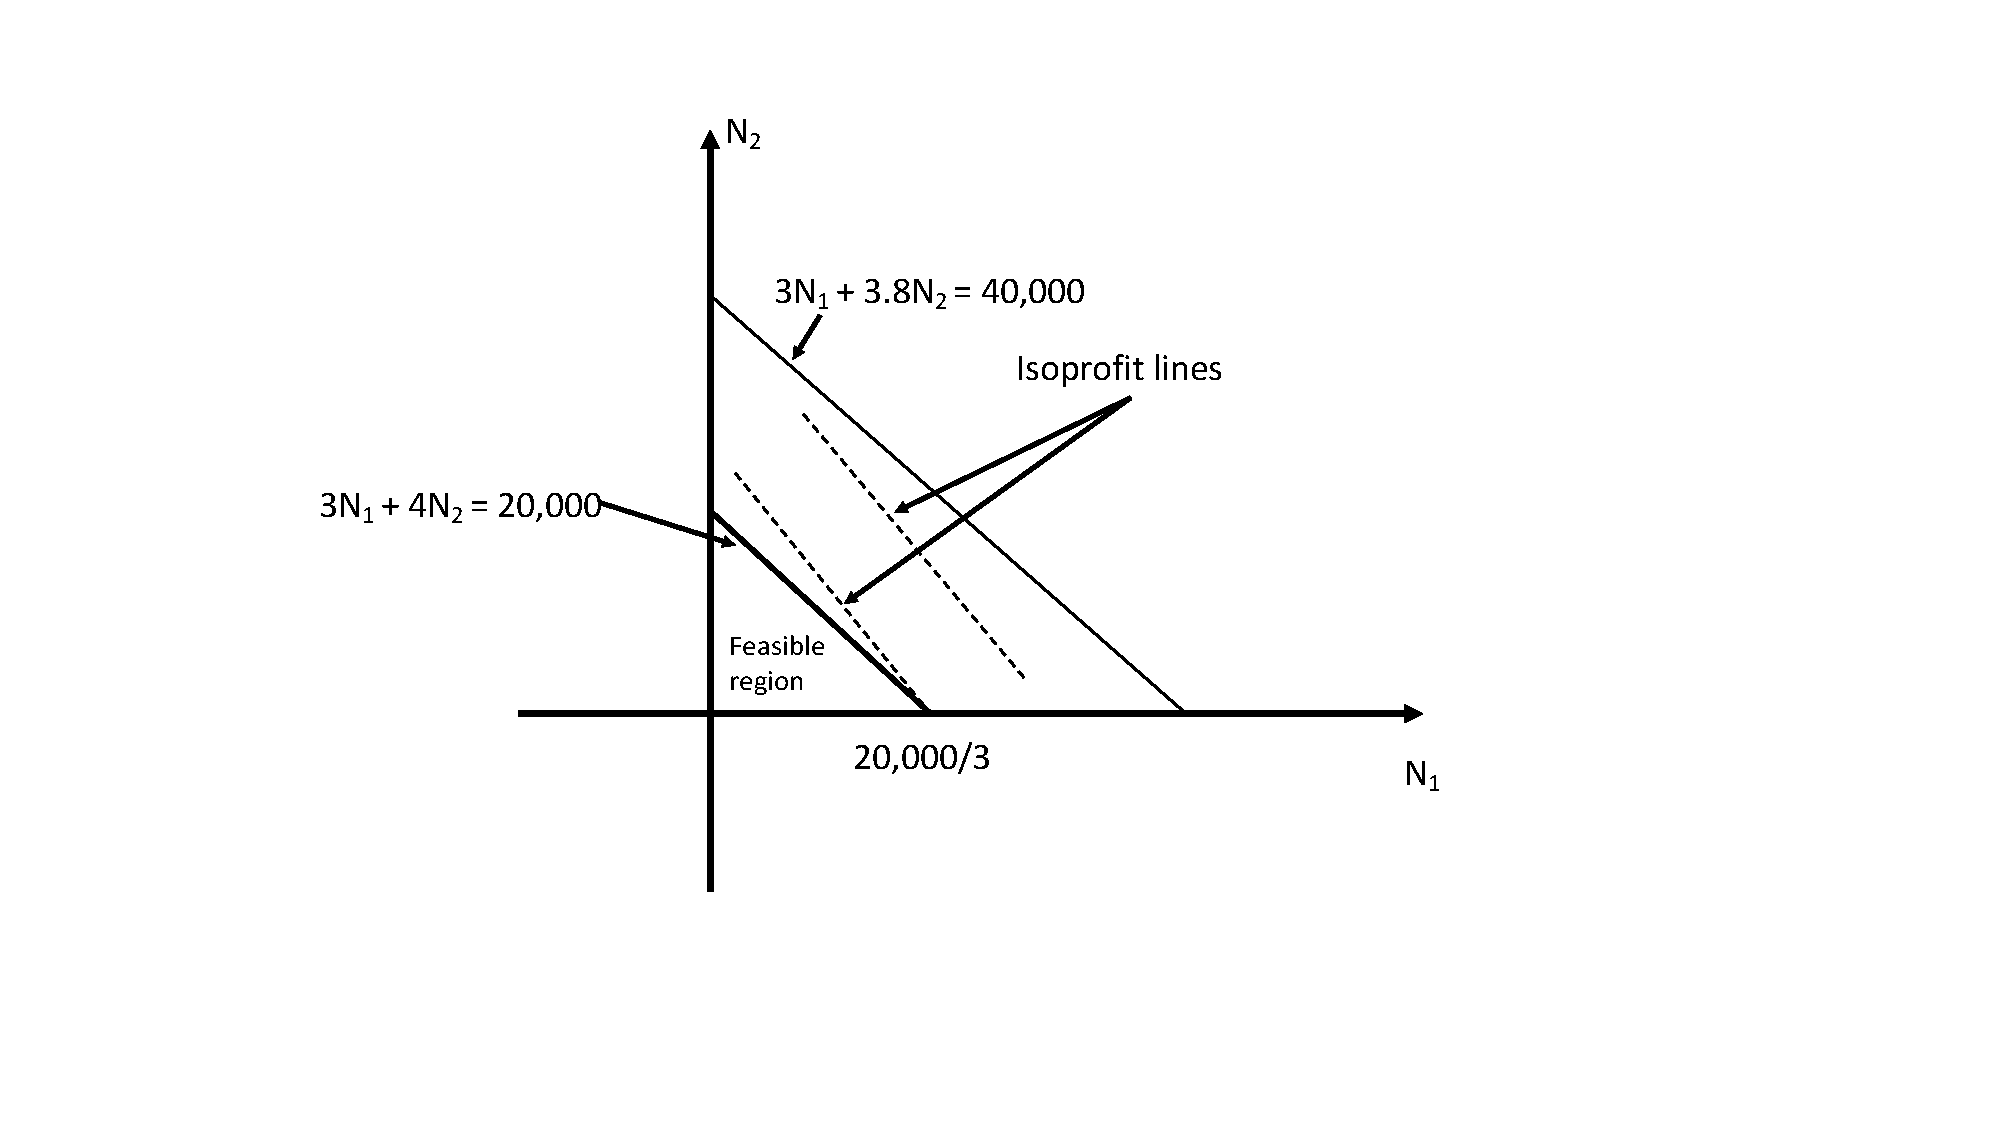
\includegraphics[width=16cm,trim={3cm 5cm 6cm 2cm},clip]{HW.pdf}
    \caption{Graphic solution to Problem 2(b).}
    \label{fig:2b}
\end{figure}

\textbf{Problem 2(c)}

If the investment is made, cash will decrease to \$3600, and machine hours will increase to  22,000. Thus, the new linear programming problem is
\begin{align*}
    \text{maximize} \quad & 3N_1 + 3.4N_2  \\
    \text{subject to} \quad & 3N_1 + 4N_2 \le 22,000 \\
    & 3N_1 + 3.8N_2 \le 36,000 \\
    & N_1 \ge 0 \\
    & N_2 \ge 0
\end{align*}

The optimal solution for the new problem is $N_1=22,000/3$, $N_2=0$, and the object function value there is 22,000. Because the maximal net income after investment (= \$22,000) is greater than that before investment (= \$20,000), the investment should be made.

\vspace{\baselineskip}
\noindent
\textbf{Problem 3.}

\noindent
\textbf{Lemma 1.} If $A\in \mathbb{R}^{m\times n}$ and $m<n$, $Ax=0$ has infinite many solutions.

\noindent
\emph{Proof.} Using the Gauss-Jordan method, we can convert $Ax=0$ to its "reduced row-echelon form", where at least $(n-m)\ge 1$ unknowns can have arbitrary values and any arbitrary value of those unknowns corresponds to a solution of $Ax=0$. Therefore, $Ax=0$ has infinite many solutions.

\vspace{\baselineskip}
Suppose that $Ax=b$ has at least one solution $x_0$. Let $S$ be the solution set of $Ax=b$. Then
\begin{gather*}
    \left\{x_0+v \;|\; Av=0 \right\} \subseteq S
\end{gather*}
where $\left\{x_0+v \;|\; Av=0 \right\}$ has infinite many elements, because $Ax=0$ has infinite many solutions (lemma 1). Therefore, $Ax=b$ has infinite many solutions.

Therefore, $Ax=b$ either has no solution at all, or has infinite many solutions.

\vspace{\baselineskip}
\noindent
\textbf{Problem 4.}

Prove that after each of the three types of row operations, the rows of the new matrix are still linearly independent. Let $r_1, r_2, r_3, ... , r_m$ be the rows of $A$. 

\vspace{\baselineskip}
\textbf{Type 1. Multiplying a row by a nonzero number.}

Suppose that after one type 1 row operation, the $i$th row of the new matrix is $kr_i$ ($k\ne 0$). 

Suppose that the rows of the new matrix are linearly dependent. Then, $\exists a_1, a_2, a_3, ... , a_m \in \mathbb{R}$, not all 0, such that
\begin{gather*}
    a_1r_1 + a_2r_2 + ... + a_i(kr_i) + ... + a_mr_m = 0
\end{gather*}

Let
\begin{align*}
    b_p=
    \begin{cases}
    a_p & p=1,2, ... ,m \text{~and~} p \ne i \\
    ka_p& p = i
    \end{cases}
\end{align*}

Then
\begin{gather*}
    b_1r_1 + b_2r_2 + ... + b_mr_m = 0
\end{gather*}
where $b_1, ... ,b_m$ are not all 0 (because $a_1, ... , a_m$ are not all 0 and $k\ne 0$). This contradicts with that the rows of $A$ are linearly independent.

Therefore, the rows of the new matrix after a finite number of type 1 row operations are still linearly independent.

\vspace{\baselineskip}
\textbf{Type 2. Adding a multiple of one row to another row.}

Suppose that after one type 2 row operation, the $i$th row of the new matrix is $r_i+kr_j$ ($i\ne j, k\in \mathbb{R}$). 

Suppose that the rows of the new matrix are linearly dependent. Then, $\exists a_1, a_2, a_3, ... , a_m \in \mathbb{R}$, not all 0, such that
\begin{gather}
    a_1r_1 + a_2r_2 + ... + a_i(r_i+kr_j) + ... + a_mr_m = 0
\end{gather}

Let
$$
    b_p = 
    \begin{cases}
    a_p & p=1,2, ... ,m \text{~and~} p \ne j \\
    a_j+a_ik & p = j
    \end{cases}
$$

Then
\begin{gather*}
    b_1r_1 + b_2r_2 + ... + b_mr_m = 0 \tag{2}
\end{gather*}

If $b_1, b_2, ..., b_m$ are all 0, then
\begin{gather*}
a_p = \begin{cases}
   b_p = 0 & p=1,2, ... ,m \text{~and~} p \ne j \\
   b_j - a_ik = - a_ik = 0 & p=j
   \end{cases} \tag{3}
\end{gather*}
which contradicts with that $a_1, ... , a_m $ are not all 0. Therefore, $b_1, b_2, ..., b_m$ are not all 0. Then, Equ. 2 contradicts with that the rows of $A$ are linearly independent.



Therefore, the rows of the new matrix after a finite number of type 2 row operations are still linearly independent.

\vspace{\baselineskip}
\textbf{Type 3. Switching two rows.}

It is obvious that the rows of the new matrix after a finite number of type 3 row operations are still linearly independent.

\vspace{\baselineskip}
In summary, if the rows of a matrix are linearly independent, then after a finite number of elementary row operations, the rows of the new matrix are still linearly independent.

\vspace{\baselineskip}
\noindent
\textbf{Problem 5.}

Prove that after each of the three types of row operations, the columns of the new matrix are still linearly independent. Let $r_1, r_2, r_3, ... , r_m$ be the rows of $A$ and $c_1, c_2, c_3, ... , c_n$ be the columns of $A$. 

\vspace{\baselineskip}

\textbf{Type 1. Multiplying a row by a nonzero number.}

Suppose that after one type 1 row operation, the $i$th row of the new matrix $A'$ is $kr_i$ ($k\ne 0$). Suppose that the columns of the new matrix are linearly dependent. Then $\exists x \in \mathbb{R}^n$, $x\ne 0$, such that
\begin{align*}
    & A'x=0 \\
    \Rightarrow \; & \begin{cases}
    r_px=0 & p=1,2, ... ,m \text{~and~} p\ne i \\
    kr_px=0 & p=i
    \end{cases} \\
    \Rightarrow \; & r_px=0, \quad p=1,2,...,m \quad (k\ne 0) \\
    \Rightarrow \; & Ax=0
\end{align*}
which contradicts with that the columns of $A$ are linearly independent.

Therefore, the columns of the new matrix after a finite number of type 1 row operations are still linearly independent.

\vspace{\baselineskip}

\textbf{Type 2. Adding a multiple of one row to another row.}

Suppose that after one type 2 row operation, the $i$th row of the new matrix $A'$ is $r_i+kr_j$ ($i\ne j, k\in \mathbb{R}$). 

Suppose that the columns of the new matrix are linearly dependent. Then $\exists x \in \mathbb{R}^n$, $x\ne 0$, such that
\begin{align*}
    & A'x=0 \\
    \Rightarrow \; & \begin{cases}
    r_px=0 & p=1,2, ... ,m \text{~and~} p\ne i \\
    (r_p+kr_j)x=0 & p=i
    \end{cases} \\
    \Rightarrow \; & \begin{cases}
    r_px=0 & p=1,2, ... ,m \text{~and~} p\ne i \\
    r_px = -kr_jx & p=i
    \end{cases} \\
    \Rightarrow \; & r_px=0, \quad p=1,2,...,m \quad (i\ne j) \\
    \Rightarrow \; & Ax=0
\end{align*}
which contradicts with that the columns of $A$ are linearly independent.

Therefore, the columns of the new matrix after a finite number of type 2 row operations are still linearly independent.

\vspace{\baselineskip}
\textbf{Type 3. Switching two rows.}

It is obvious that the columns of the new matrix after a finite number of type 3 row operations are still linearly independent.

\vspace{\baselineskip}
In summary, if the columns of a matrix are linearly independent, then after a finite number of elementary row operations, the columns of the new matrix are still linearly independent.

\vspace{\baselineskip}
\noindent
\textbf{Problem 6.}

\textbf{Problem 6(a)}

For any two elements $x$ and $y$ of $S_0$ and two real numbers $\alpha$ and $\beta$,
\begin{gather*}
    2 \alpha x+x_0 = 2\alpha(x+x_0) + (1-2\alpha) x_0 \in S \quad(x+x_0  \in S, x_0 \in S) \\
    2 \beta y+x_0 = 2\beta(y+x_0) + (1-2\beta) x_0 \in S \quad(y+x_0  \in S, x_0 \in S)
\end{gather*}

Therefore,
\begin{gather*}
    \alpha x + \beta y + x_0 = \frac{1}{2}(2 \alpha x+x_0) + \frac{1}{2} (2 \beta y+x_0) \in S
\end{gather*}

Therefore, $\alpha x+ \beta y \in S_0$. Therefore, $S_0$ is a subspace.

\vspace{\baselineskip}
\textbf{Problem 6(b)}

The dimension of $S$ is 3.
\begin{gather*}
S=
\begin{bmatrix} 
x_1 \\
x_1-2 \\
2x_1-3 \\
x_4 \\
x_5
\end{bmatrix}
= x_1 \begin{bmatrix} 
1 \\
1 \\
2 \\
0 \\
0
\end{bmatrix}
+x_4\begin{bmatrix} 0 \\ 0 \\ 0 \\ 1 \\ 0 \end{bmatrix}
+x_5\begin{bmatrix} 0 \\ 0 \\ 0 \\ 0 \\ 1 \end{bmatrix}
+\begin{bmatrix} 0 \\ -2 \\ -3 \\ 0 \\ 0 \end{bmatrix},
\quad x_1, x_4, x_5 \in \mathbb{R}
\end{gather*}


Let $x_0 = \begin{bmatrix} 0 & -2 & -3 & 0 & 0 \end{bmatrix}^T$, then
\begin{gather*}
S_0= S-x_0 =\text{span}(\begin{bmatrix} 
1 \\
1 \\
2 \\
0 \\
0
\end{bmatrix}, \begin{bmatrix} 0 \\ 0 \\ 0 \\ 1 \\ 0 \end{bmatrix}, \begin{bmatrix} 0 \\ 0 \\ 0 \\ 0 \\ 1 \end{bmatrix})
\end{gather*}
and the dimension of $S_0$ is 3. Thus, the dimension of $S$ is 3.

% --------------------------------------------------------------
%     You don't have to mess with anything below this line.
% --------------------------------------------------------------

\end{document}